\documentclass[letterpaper,twocolumn,10pt]{ilass}
\def\thepage{}

%\usepackage{times}
\usepackage{amssymb}
\usepackage{amsmath}
\usepackage{tikz}
\usepackage{graphicx}
\usepackage{gensymb}

\usepackage{graphicx}

\evensidemargin = 0.0in
\headheight = 0.0in
\headsep = 0.0in
\parskip = 0.0in
\parindent = 0.25in
\topmargin    0.00in
\oddsidemargin 0.00in
\textheight    9.00in
\textwidth     6.50in
\columnsep     0.25in

\title{\vspace{-0.25in}
      {\small \em
       ILASS-Americas 29th Annual Conference on Liquid Atomization and Spray Systems,
       Atlanta, GA, May 2017} \newline\newline
      {\large\bf In-Nozzle Flow Investigations of Marine Diesel Injectors} }
				
\author{\large
        R. Balz\textsuperscript{1,2}\footnote{reto.balz@wingd.com},
				D. Sedarsky\textsuperscript{1},
				and A. Schmid\textsuperscript{2}\\
				%
				\textsuperscript{1}Chalmers University of Technology, Combustion Division,
				G\"oteborg, Sweden\\
				%
				\textsuperscript{2}Winterthur Gas \& Diesel Ltd., Winterthur,
				Switzerland}

\date{\normalsize  \centerline{\bf Abstract} \vspace{0.05in}
\begin{minipage}{6.5in} \normalsize
Injector geometries of large marine two-stroke diesel engines differ extensively from
configurations typically used in diesel engines for automotive applications.
The injector orifices are arranged asymmetrically, as all the bores face a similar direction.
Due to this setup, the orifices are also distributed eccentric with respect to the central axis
of the injector. Experiments have shown that sprays from such orifices propagate non-symmetrical
to the nominal axis of the orifice. Those spray deviations can lead to wall wetting which
increases fuel consumption, emissions, component temperatures and loss of lubrication film.
To further investigate the in-nozzle flow and how it affects the spray morphology for large
marine two-stroke diesel engine injectors, experiments were performed using transparent nozzles
made of PMMA and real condition injection pressures and air densities of up to 80~MPa and
35~kg/m$^3$, respectively. The experiments were performed with diesel fuel in a newly built
spray chamber to cope with the spray backsplash under ambient temperature conditions.
The nozzle used was an orthogonally arranged 0.75~mm diameter one-hole setup that matches large
marine two-stroke diesel engines injector nozzle diameters. High-speed shadowgraphie using a
far-field microscope was applied to visualize the cavitation in the nozzle during the complete
injection process.
The evaluation of cavitation regions in the nozzle with various Cavitation numbers delivers
valued validation data for cavitation CFD models.
\end{minipage} \vspace{-0.25in}}
\baselineskip = 2.0\baselineskip

\begin{document}

\ifpdf
\DeclareGraphicsExtensions{.pdf, .jpg}
\else
\DeclareGraphicsExtensions{.eps, .jpg}
\fi

\maketitle

\clearpage

\pagenumbering{arabic}
\setcounter{page}{2}


%INTRODUCTION
\section*{Introduction} 
Much of the ongoing marine engine development is focused on meeting the requirements of the
IMO (organisation maritime internationale) Tier III legislation. Tier III dictates an 80\%
reduction in $NO\textsubscript{x}$ engine out levels. Engine manufacturers are investigating
engine internal $NO\textsubscript{x}$ reduction methods such as Miller/Atkinson timing, water
in fuel emulsion, and EGR (exhaust gas recirculation). The development of these methods requires
that engine manufacturers have a good understanding of all the internal engine processes,
including fuel injection.\\
%
Winterthur Gas \& Diesel Ltd. (hereinafter reffered to as Win~G\&D) is a leading developer of
low-speed gas and diesel engines used for propulsion power in merchant shipping. The company 
has a unique constant volume spray combustion chamber (SCC) of dimensions representative of
smaller two-stroke marine engines (\o 500 x 150~mm) \cite{Herrmann2011}. Investigations on the
SCC have shown that the highly non-symmetrical and eccentric nozzle designs of large two-stroke
marine engines have spray deflections in the range of 10$^{\circ}$ \cite{Schmid2013}. Further
studies, including CFD simulations with an advanced cavitation model, show how the two-phase,
highly compressible flow inside the nozzle influences the spray propagation. The results
indicate that cavitation plays a large role in the development of the spray \cite{Schmid2014}.
Cavitation can occur as "geometric cavitation" (located at the corner and wall of the nozzle
hole and caused by the sudden reduction of static pressure as the flow enters the passages)
or as "string cavitation" (sometimes called “vortex cavitation”, appearing transiently within
the core of strong vortices that can build up in these geometries) \cite{Andriotis2008}.
It appears that both types of cavitation can occur in the kind of injector used in large
two-stroke marine diesel engines. It is not clear how switching from one type of internal
flow to another will affect spray formation and thus spray breakup, mixing and combustion
in a real marine engine during one cycle.\\
%
The detailed understanding of the flows in the interior of the nozzle and their effect on fuel
spray formation (primary breakup) remains a weak link in CFD modeling of large two-stroke marine
engines. Additionally, primary breakup is the least understood part of the spray combustion
process \cite{Fansler2015,Linne2013}. The Combustion Division of Chalmers University of
Technology (hereinafter referred to as Chalmers) has recently developed an optically
transmissive injector tip that can withstand higher fuel pressures than former designs
\cite{Falgout2015}. By adapting the Win~G\&D nozzle geometries to the transparent nozzle
holder from Chalmers, in-nozzle flow investigations under engine-like conditions can be
realized to help validate cavitation models to achieve better CFD predictability of the
whole injection process.\\
%
In-nozzle flow has been extensively researched with transparent nozzles or ionizing radiation,
for real-size and scaled geometries but mostly for small engine injectors as used for cars and
trucks \cite{Fansler2015, Blessing2003, Duke2014}.
\cite{Hult2016} showed in-nozzle flow measurements for large marine diesel engines but at
reduced fuel pressures around 10~MPa for real-size nozzle geometries. Additionally, a
diesel surrogate, an oil with a similar refractive index, has been used.
The aim of this study is to generate validation material for CFD cavitation models by
using simplified but real-size nozzle geometries under engine-like conditions of marine
diesel engines. 

%NEW SPRAY CHAMBER
\section*{New spray chamber}
A large spray chamber has been designed and built to deal with the rebounding fuel spray.
This is a problem as the nozzle dimensions and therefore fuel flow are extensively higher
than in smaller engines. 

\begin{figure}[h]
\begin{center}
\begin{tikzpicture}
\node[inner sep=0pt] (russell) at (0,0){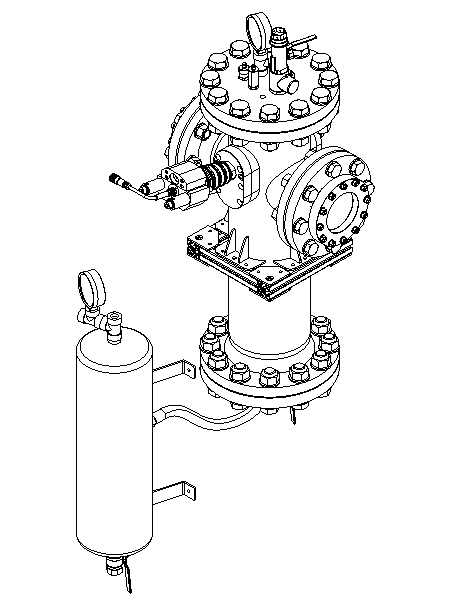
\includegraphics[width=3in]{mark7_ill_iso_1}};
\draw (-0.94in,1.34in) node[]{a};
\draw[dashed] (-0.89in,1.31in) -- (-0.42in,0.87in);
\draw (-0.54in,0.24in) node[]{b};
\draw[dashed] (0.03in,0.05in) -- (-0.49in,0.21in);
\draw (-1.33in,0.19in) node[]{c};
\draw[dashed] (-0.98in,-0.3in) -- (-1.3in,0.16in);
\draw (0.20in,-1.01in) node[]{d};
\draw[dashed] (0.01in,-0.86in) -- (0.16in,-0.99in);
\draw (-0.17in,-1.82in) node[]{e};
\draw[dashed] (-0.64in,-1.79in) -- (-0.22in,-1.82in);
\draw (1.23in,0.40in) node[]{f};
\draw[dashed] (0.76in,0.59in) -- (1.19in,0.4in);
\draw (1.09in,1.69in) node[]{g};
\draw[dashed] (0.42in,1.56in) -- (1.06in,1.7in);
\end{tikzpicture}
\end{center} 
\vspace*{-5mm}
\caption{Isometric view schemata of new spray chamber:
         a) Win~G\&D injector,
				 b) spray chamber,
				 c) auxilliary tank,
				 d) connection hose,
				 e) drainage valve,
				 f) fused silica window,
				 g) safety relief valve and accessories.}
\label{fig1} 
\end{figure}

Therefore, most existing spray chambers are too small for marine engine spray investigations.
Nozzle diameters for large two-stroke diesel engines can have diameters larger than 1 mm.\\
%
The design of the newly built spray chamber at Chalmers is based on standardized stainless
steel flanges for pipes (EN 1092-1) that are welded to the spray chambers main body,
a stainless steel pipe with a diameter of approximately 200~mm. The standard flanges allow
maximal versatility at very low cost. A schematic of the spray chamber is depicted in figure
\ref{fig1}. The spray chamber is designed for ambient temperatures as its main purpose is the
use of injectors with transparent nozzles made of PMMA, a thermoplast with a low melting point
around 140 to 160$^{\circ}$C. As the goal is to investigate the in-nozzle flow and how 
affects the primary breakup of the spray, it is assumed that the surrounding gas density plays
the dominant role and therefore the temperature can be neglected. The spray chamber can be
filled with nitrogen or air to pressures up to 3~MPa to match engine-like air densities at
ambient temperatures which are around 35~kg/m$^3$. The system includes an auxiliary pressure
vessel that allows flushing the content of the spray chamber into it (see figure \ref{fig1}).
This process is necessary to deal with the large amount of fuel that is injected into the
spray chamber and to maintain maximal visibility by reducing precipitation of the fine fuel
droplets on the windows. The auxiliary tank is mounted at a lower position as depicted in
figure \ref{fig1} to also collect the accumulated fuel. A pneumatically driven angle valve
is used to control the flushing. The valve is mounted at the bottom flange of the spray
chamber and not visible in figure \ref{fig1}. 

\begin{figure}[h]
\begin{center}
\begin{tikzpicture}
\node[inner sep=0pt] (russell) at (0,0){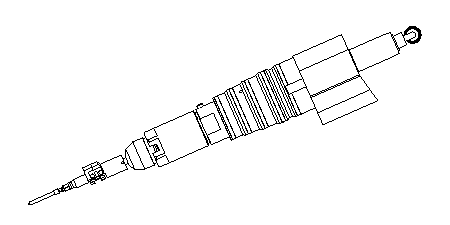
\includegraphics[width=3in]{injector_ill_1}};
\draw (0.21in,0.75in) node[]{a};
\draw[dashed] (0.16in,0.23in) -- (0.2in,0.7in);
\draw (-0.75in,0.3in) node[]{b};
\draw[dashed] (-0.78in,-0.32in) -- (-0.75in,0.25in);
\draw (-1.32in,0.05in) node[]{c};
\draw[dashed] (-1.05in,-0.475in) -- (-1.3in,0in);
\end{tikzpicture}
\end{center}
\vspace*{-5mm}
\caption{Schemata of injector setup:
         a) Win~G\&D injector,
				 b) transparent nozzle holder,
				 c) Kistler pressure sensor.}
\label{fig2} 
\end{figure}

The spray chamber is mounted on a rig and the control and sensor signals are collected in an
electrical box where a simple connection to the data acquisition hardware can be setup, so
that the spray chamber as a whole rig can be easily moved. 
Pressure and temperature sensors are installed to control the desired air density conditions
within the spray chamber and control the filling and flushing procedures.\\
%
Line-of-sight optical access is provided by two fused silica windows with optically usable
diameters of 120~mm. Fused silica is used over cheaper technical glass that is thermally
pre-stressed and therefore interferes with the lights polarization. This is important as
change of polarization is used as shutter for the ballistic imaging optical measurement
technique that will be applied later in the project \cite{Linne2013}. The windows are clamped
onto modified standard flanges as depicted in figure \ref{fig1}. Two flanges that are
orthogonally arranged with respect to the optical access are used as dummy and for the
injector mount, respectively. \\
%
The injector is mounted with an angle to additionally reduce rebounding of the spray by
aiming it with a flat angle to the spray chambers inner wall. The flanges are compatible
to the high-pressure, high-temperature spray chamber at Chalmers to guarantee maximal
compatibility for further use of the spray chamber. The mounted injector is provided
by Win~G\&D and its nozzle adapted so that the transparent nozzle holder can be mounted
(see figure \ref{fig2}). To cope with the need for high diesel mass flows for the marine
injectors, a piston accumulator with a total volume of 5~dm$^3$ has been used to stabilize
the injection pressure over the injection duration of approximately 8~ms. 


%EXPERIMENT
\section*{Experimental setup}
National Instruments hardware and LabVIEW have been used to control the experiments.
A shadowgraphy optical setup has been arranged using a Vision Research Phantom V1210
12-Bit high-speed camera, a far-field microscope form LaVision and a Cavilux Smart
diode laser from Cavitar, emitting at 640~nm. The images where recorded at a framerate of
20,000~fps and a resolution of 512~x~800~pixels which is equal to a field of view (FOV)
of approximately 2.5 x 3.9~mm (see figure \ref{fig3}). 

\begin{figure}[h]
\begin{center}
\begin{tikzpicture}
\node[inner sep=0pt] (russell) at (0,0){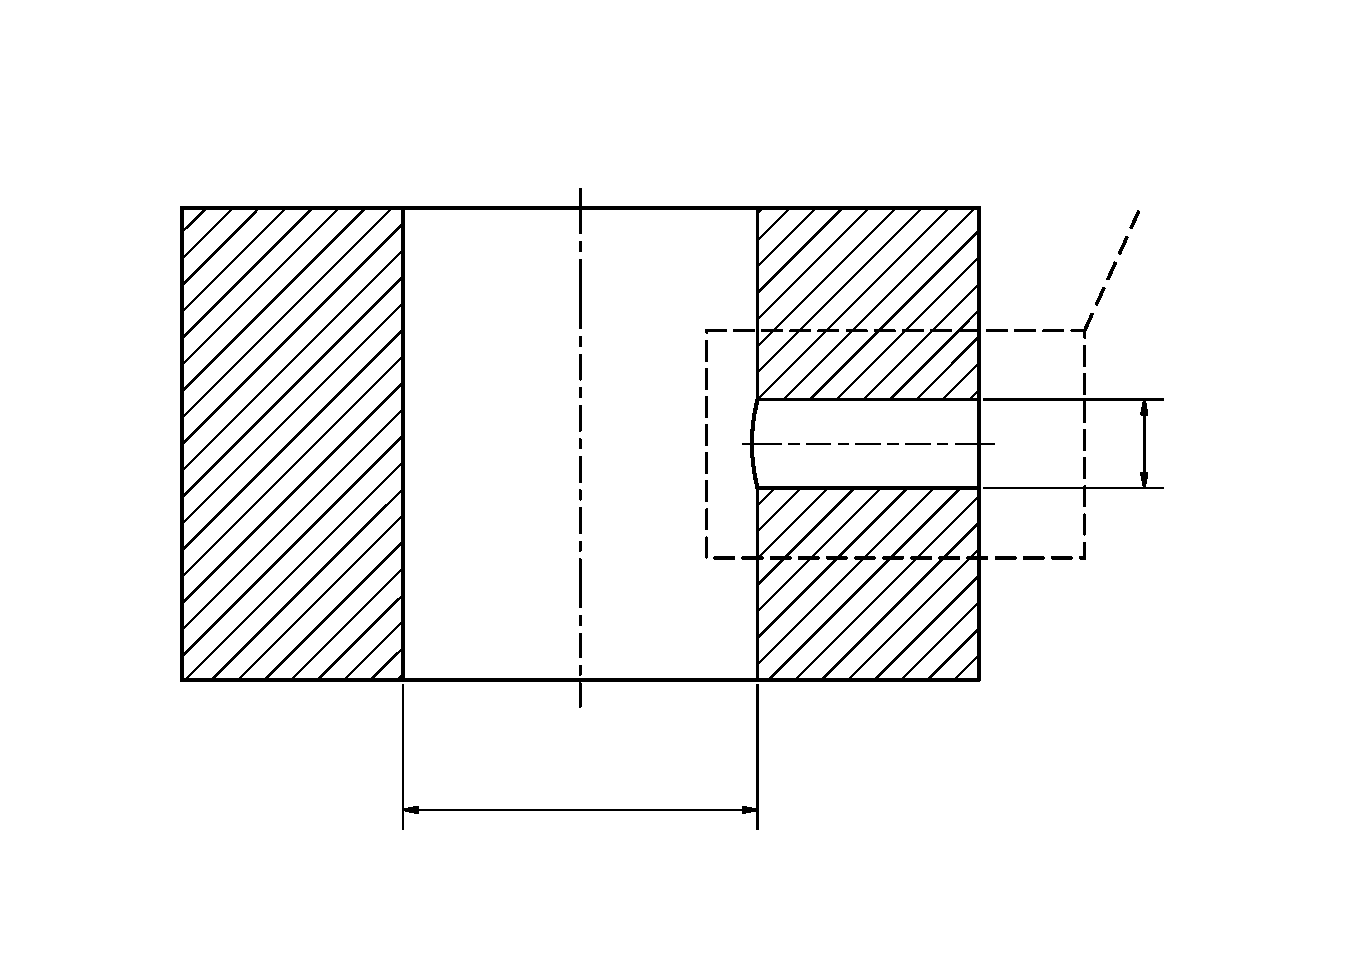
\includegraphics[width=3in]{nozzle_ill}};
\draw (0.98in,0.07in) node[rotate=90]{\o a};
\draw (-0.21in,-0.67in) node[]{\o b};
\draw (1.03in,0.67in) node[]{FOV};
\end{tikzpicture}
\end{center}
\vspace*{-10mm}
\caption{Section view of transparent nozzle made of PMMA with orifice diameter
         \o a = 0.75~mm and sac diameter \o b = 3~mm. The field of view (FOV)
				 of the optical setup used is illustrated as dashed rectangle.}
\label{fig3} 
\end{figure}

A Kistler piezo-resistive pressure sensor with a natural frequency over 200~kHz has been used
together with a National Instruments USB-6351 DAQ with 1.25~MS/s to measure the fuel pressure
close to the transparent nozzle. The location of the pressure sensor is depicted in figure
\ref{fig2} c). The close position to the nozzle allows for accurate pressure measurements as
fuel injectors usually have high pressure loss. Accurate pressure information close to the
orifice is of high value for setting boundary conditions in CFD simulations. \\
%
The transparent nozzle holder has been developed at Chalmers \cite{Falgout2016}. The used nozzle
geometry is shown in figure \ref{fig3}. For the first investigations the nozzle design has been
chosen to be simple, viz. perpendicular, sharp edges and no taper. The nozzle used has a sac
diameter of 3~mm (see figure \ref{fig3},  {\o b}) and the orifice has a diameter of 0.75~mm
(see figure \ref{fig3},  {\o a}) and a length of 1.875~mm.
PMMA is used as transparent nozzle material as it has a very similar refractive index as
diesel fuel. This index matching allows visualization of the in-nozzle flow with no optical
distortion from the round orifice geometry. The diesel fuel used has a density of
815.9~kg/m$^3$ (at 20$^{\circ}$C) and a viscosity of 2.112~mm$^2$/s (at 40$^{\circ}$C).\\
%
The high static pressure applied to the PMMA nozzles allows only a limited number of injections
before failure \cite{Falgout2016}. This has the advantage that wear of the nozzle can be
neglected, but the experimental effort is higher as the nozzles have to be replaced in short
intervals which is also combined with aligning and focusing of the optical setup. As every
nozzle geometry is slightly different due to manufacturing tolerances, a statistical error
in the measurements is induced. The short life expectancy of the PMMA nozzles at high fuel
pressures makes nozzle characterization measurements like impingement force evaluation
disputable as these evaluations need a high number of injections to be accurate.\\
%


%RESULTS
\section*{Results}
Literature uses different non-dimensional cavitation numbers ($CN$) to represent cavitation
conditions in nozzles. These numbers are usually defined as ratios from pressure in front and
behind the orifice and the vapour pressure of the liquid \cite{Hult2016, Giannadakis2008}.
A commonly used one is
$(p\textsubscript{i} - p\textsubscript{b})/(p\textsubscript{b}-p\textsubscript{v})$,
where $p\textsubscript{i}$ is the pressure upstream and $p\textsubscript{b}$ the pressure
downstream the orifice (also called back pressure). $p\textsubscript{v}$ is the vapor pressure
of diesel and neglected as insignificant for $CN$ when using rail pressures orders of magnitude
higher.\\
%
All images shown are acquired during the quasi-steady state condition of the injection, where
the needle of the injector is open and therefore the fuel pressure and volume flow is
approximately constant. Figure \ref{fig4} a) and b) show the cavitation flow at 50~MPa rail
pressure and an air density of 1.2~kg/m$^3$ ($CN \approx 390$). Dark areas within the nozzle
indicate gaseous and bright areas liquid aggregate state of the diesel fuel. By comparing the
schematic sketch of the nozzle in figure \ref{fig3} and the images shown
(e.g. in figure \ref{fig4}) the selected FOV can be interpreted. The flow direction of the
diesel fuel is from top. It enters the orifice and flows to the right where at the end of the
orifice the spray emerges.


\begin{figure}[h]
\begin{center}
\begin{tikzpicture}
\node[inner sep=0pt] (russell) at (0,0){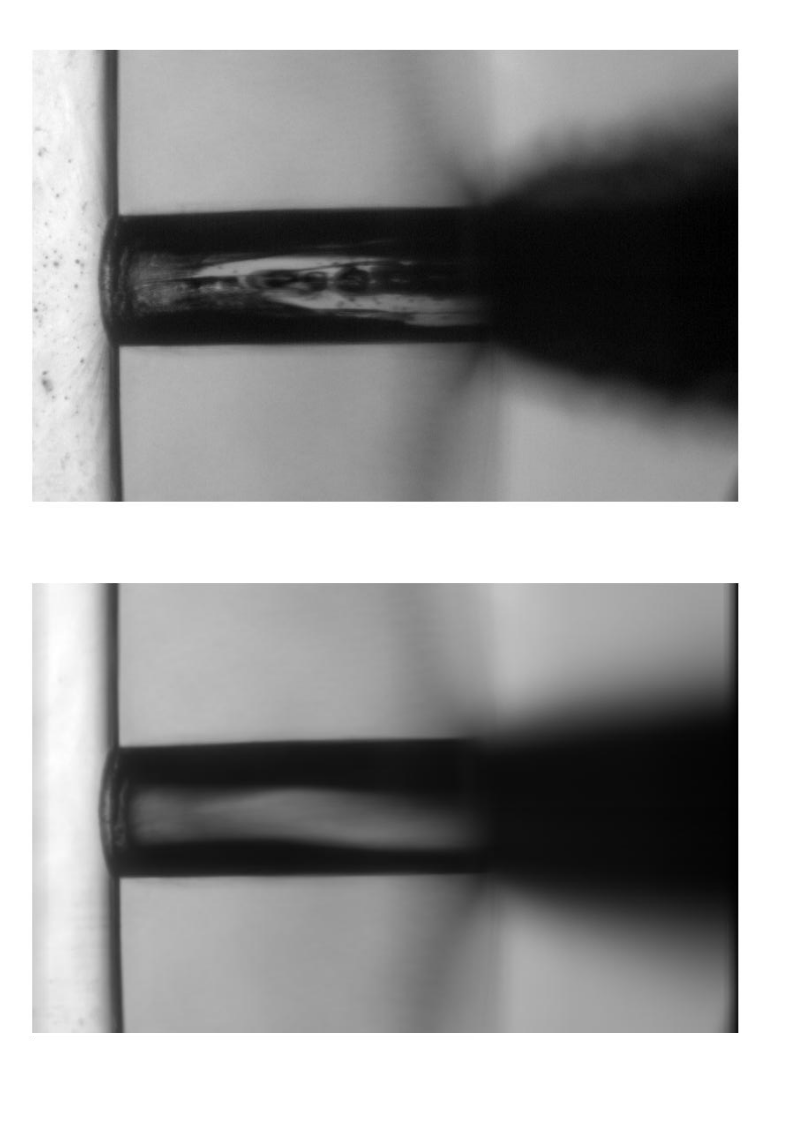
\includegraphics[width=3in]{Zeichnung.png}};
\draw (1.45in,-1.7in) node[]{b)};
\draw (1.45in,0.3in) node[]{a)};
\end{tikzpicture}
\end{center}
\vspace*{-10mm}
\caption{Cavitation in orifice at 50 MPa rail pressure and atmospheric back pressure
         ($CN \approx 390$): a) single shot image with transient, turbulent cavitation
				 phenomena in the orifice center, b) averaged image.}
\label{fig4} 
\end{figure}


The spray that emerges the orifice of the transparent nozzle is unsharp as it is out of the
focus plane. The dark vertical line on the left side of the image indicates the sac hole wall.
This line is visible as the refractive index of the used diesel fuel and the PMMA is very
similar but not completely identical.\\


\begin{figure}[h]
\begin{center}
\begin{tikzpicture}
\node[inner sep=0pt] (russell) at (0,0){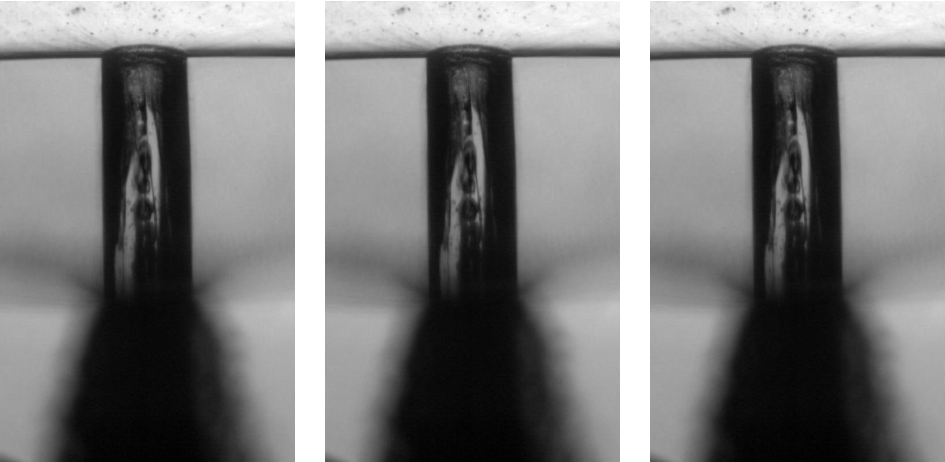
\includegraphics[width=3in]{3_Bild_test}};
\end{tikzpicture}
\end{center}
\vspace*{-2mm}
\caption{Cavitation in orifice at 50 MPa rail pressure and different back pressures of
         1~atm (left), 1.5~MPa (middle) and 3~MPa (right). Note that the images are
				 rotated clockwise by 90$^{\circ}$ compared to figure \ref{fig3} and \ref{fig4}.}
\label{fig5} 
\end{figure}


The cavitation pockets along the orifice walls emerge over the whole length. It can be assumed
that for this setup a non-symmetrical hydraulic flip state describes the cavitation the best.
However, the cavitation is highly unsymmetrical as clearly visible in the averaged image shown
in figure \ref{fig4} b). The cavitation pocket on the top side of the orifice is larger which
can be explained with the flow direction coming from the top of the sac bore.\\
%
To eliminate the transient turbulence phenomena in the orifice, the acquired single images
during the steady-state injection process have been averaged over multiple injections. An
averaged image is depicted in figure \ref{fig4} b).\\
%
The transient cavitation phenomena that are visible between the cavitation pockets along the
orifice walls are highly fluctual and different from image to image.  As the images are only
acquired with 20,000~fps the timing between single events is 50~$\mu$s which is too long at
the given velocities to connect the transient events together for further evaluation
(e.g. velocity information).\\
%
Figure \ref{fig5} shows the averaged in-nozzle flow with identical rail pressure (50~MPa)
for different back pressures: 1~atm ($CN \approx 390$), 1.5~MPa ($CN \approx 25$) and 3~MPa
($CN \approx 12$)). The images are rotated clockwise by 90$^{\circ}$ compared to figure
\ref{fig3} and \ref{fig4}. The flow enters the nozzle from the right side and leaves the
orifice to the bottom. The cavitation pocket sizes get smaller with increasing back pressure
(decreasing $CN$) but remain filling the whole length of the orifice on both sides.\\
%
The in-nozzle flow depicted in figure \ref{fig6} is an averaged image from injections at
80~MPa rail and 3~MPa back pressure ($CN \approx 21$). This pressure ratio represents the
same fuel pressure and air density as in large two-stroke marine diesel engines.\\
%


\begin{figure}[h]
\begin{center}
\begin{tikzpicture}
\node[inner sep=0pt] (russell) at (0,0){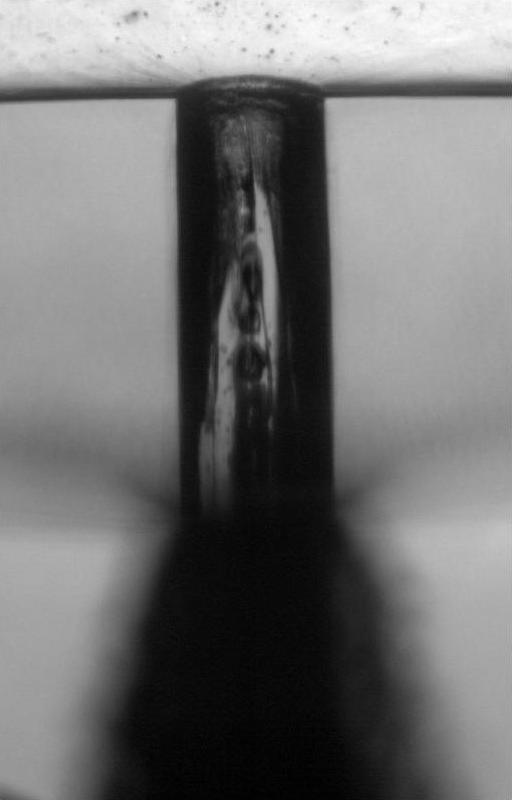
\includegraphics[angle=90, width=3in]{20170227_02_0165_edit}};
\end{tikzpicture}
\end{center}
\vspace*{-2mm}
\caption{Cavitation in orifice at 80 MPa rail pressure and 3~MPa back pressures ($CN \approx 21$).}
\label{fig6} 
\end{figure}


Similar to the images shown from lower injection pressure (see figure \ref{fig4} and \ref{fig5}),
the cavitation emerges over the whole length of the orifice as well.\\
%
The cavitation number for the shown cases at 50~MPa (1.5~MPa back pressure) and 80~MPa
(3~MPa back pressure) rail pressure are similar ($CN \approx 25$ and $CN \approx 21$,
respectively) but the cavitation pockets within the orifice look different when compared
to each other.\\



%CONCLUSIONS
\section*{Conclusions}
The newly developed spray chamber proofs to be a valuable addition to the experimental equipment
at Chalmers. The flushing procedure helps reduce fuel deposits on the windows significantly.
The transparent nozzle holder developed by \cite{Falgout2015} was able to withstand the desired
fuel pressures of up to 80~MPa and the large orifice diameter of 0.75~mm. However, due to space
limitations of the current design, a new transparent nozzle holder has to be developed.
Especially for angled orifices and multi-hole nozzles, the current design is not feasible due
to geometrical restrictions. Additionally, to investigate the transient in-nozzle flow at the
start of injection when the needle in the injector is moving, the design has to be altered to
fit to the non-sac Win~G\&D injectors.\\
%
The qualitative, averaged, quasi-steady state cavitation images can be reproduced with different
PMMA nozzles from the same manufacturing batch. It can therefore be assumed that the
manufacturing tolerances play an unimportant role for the used design.\\
%
The acquired images show small bubbles in the sac bore. Experiments show that the temperature
and the amount of disolved gas in the fuel change the cavitation pocket size \cite{Watanabe2014}.
It has therefore to be investigated how the amount of dissolved gas in the diesel used and
the fuel properties itself alters the cavitation properties. It also has to be investigated
how the fuel temperature changes the in-nozzle flow regarding cavitation. This could be realized
by tempering the Win~G\&D injector to different temperatures (in temperature ranges where the
durability of the used thermoplast PMMA is still guaranteed).\\
%
The strongly developed cavitation flow as depicted in the images can be attributed to the
sharp edge design of the nozzle. As this sharp edge between sac bore and orifice is not
realistic for commercial injectors (as usually radii are machined by either electrochemical
machining or hydro-erosive grinding), nozzle geometry variations (inlet radius, taper and angle)
will be investigated in future work.\\
%
Additionally, simultaneous optical measurements of in-nozzle flow and primary spray breakup
will be the next step in this project as well as first CFD validation within the simulation
groups at Win~G\&D and Combustion Division at Chalmers.\\
%



%ACKNOWLEDGMENT
\section*{Acknowledgment}
The authors would like to thank the Combustion Engine Research Center (CERC),
the Swedish Energy Agency and the Swiss Federal Office of Energy for funding.
Special thanks to Mark~Linne and Zachary Falgout for their support.
\newline

%REFERENCES
\bibliography{ilass}
\bibliographystyle{ilass}

\end{document}
\end

